\chapter{Obtained data analysis} \label{chap:seven}
This chapter will discuss what can be done with the data obtained from the simulations. In \autoref{sect-7.1}, we will introduce the data analysis tool able to generalise data of many participants and extract locations where violations occurred. The \autoref{sect-7.2} will present two ways the analysed data can be depicted visually, mainly via diagrams and location marking on the map. The chapter is finished in \autoref{sect-7.3} after introducing a script calculating the safety performance score of a driver in a particular scenario building on the concepts discussed in \autoref{sect-6.3}.

\section{The data analysis tool} \label{sect-7.1}
Let us begin by discussing how the data obtained from the simulations could be processed. This article proposes an easily customisable way to perform data analysis that suits the user's needs. An overview of the analysis process can be seen in \autoref{fig:data_analysis}.

\begin{figure} [h]
    \centering
    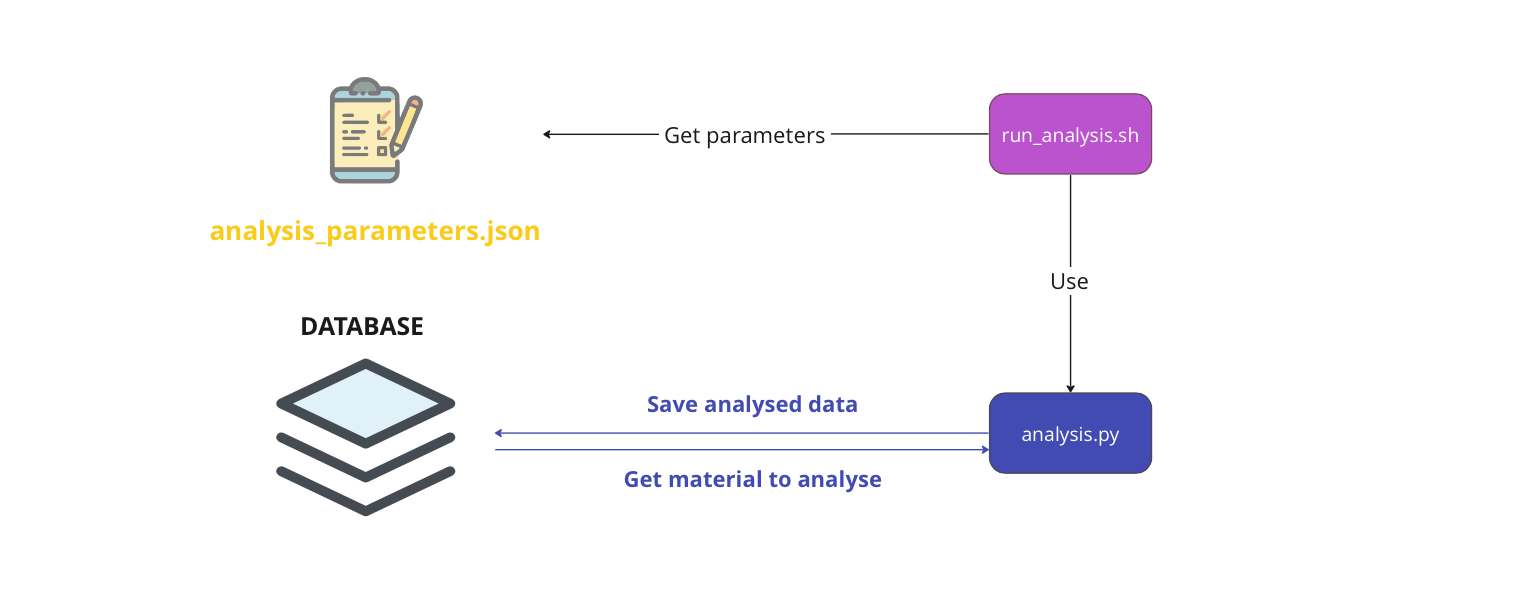
\includegraphics[width = \textwidth]{research_paper/Images/data_analysis.png}
    \caption{An overview of data analysis}
    \label{fig:data_analysis}
\end{figure}

Here the user specifies the parameters in the analysis\_parameters.json file and runs the run\_analysis.sh script, which takes the necessary data from the database, performs the analysis and saves the analysed data back to the database in a new folder whose name is specified by the user. An example of what the analysis\_parameters.json file looks like can be seen in \autoref{fig:analysis_parameters} in \autoref{chap:a}. In the file, the user specifies which participants, scenarios and safety metrics must be analysed. The algorithm then performs the analysis and stores the data that can be divided into three categories: the overall performance of participants in the scenarios (stored in participants.xml file), the average scenario scores of the participants (stored in scenarios.xml file) and files with locations of where the violations occurred (stored in separate files in points directory). To deepen the understanding of the analysed data, the reader is highly encouraged to have a look at an example of data analysis in data/analysed\_data/data/example\_analysis directory.

\section{Visualising the data} \label{sect-7.2}

Now that we have introduced a way of analysing the data and described the basic principles, it is time to see how analysed data can be put in a visual format for further analysis. The overview of the visualisation methods can be seen in \autoref{fig:visualisation}.

\begin{figure} [h]
    \centering
    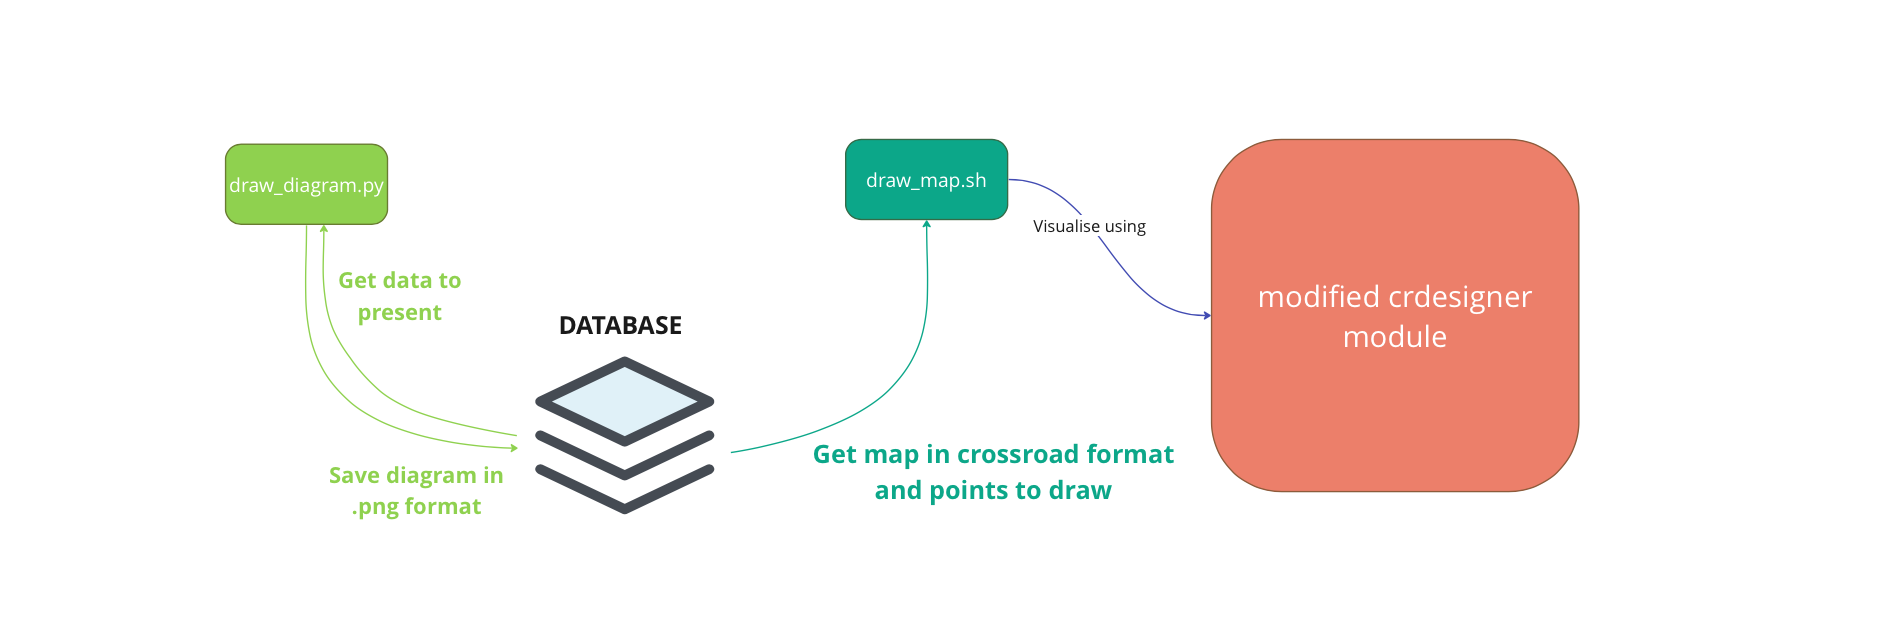
\includegraphics[width = \textwidth]{research_paper/Images/visualisation.png}
    \caption{Data visualisation process}
    \label{fig:visualisation}
\end{figure}

The last section mentioned that the data analysis tool creates three types of processed data: participant analysis, scenario analysis and metrics analysis. The first two categories can be used to draw diagrams indicating the general tendencies. An example of the diagram can be seen in \autoref{fig:diagram_example}. The diagram displays the amount of penalty points each participant received for collisions in scenario 1. The information can help compare participants, including the AI implementations, in different scenarios. Similar diagrams can be generated to compare the scenario scores concerning different metrics. For instance, to compare which scenarios were more prone to traffic rule violations or breaches of other safety metrics.

\begin{figure} [h]
    \centering
    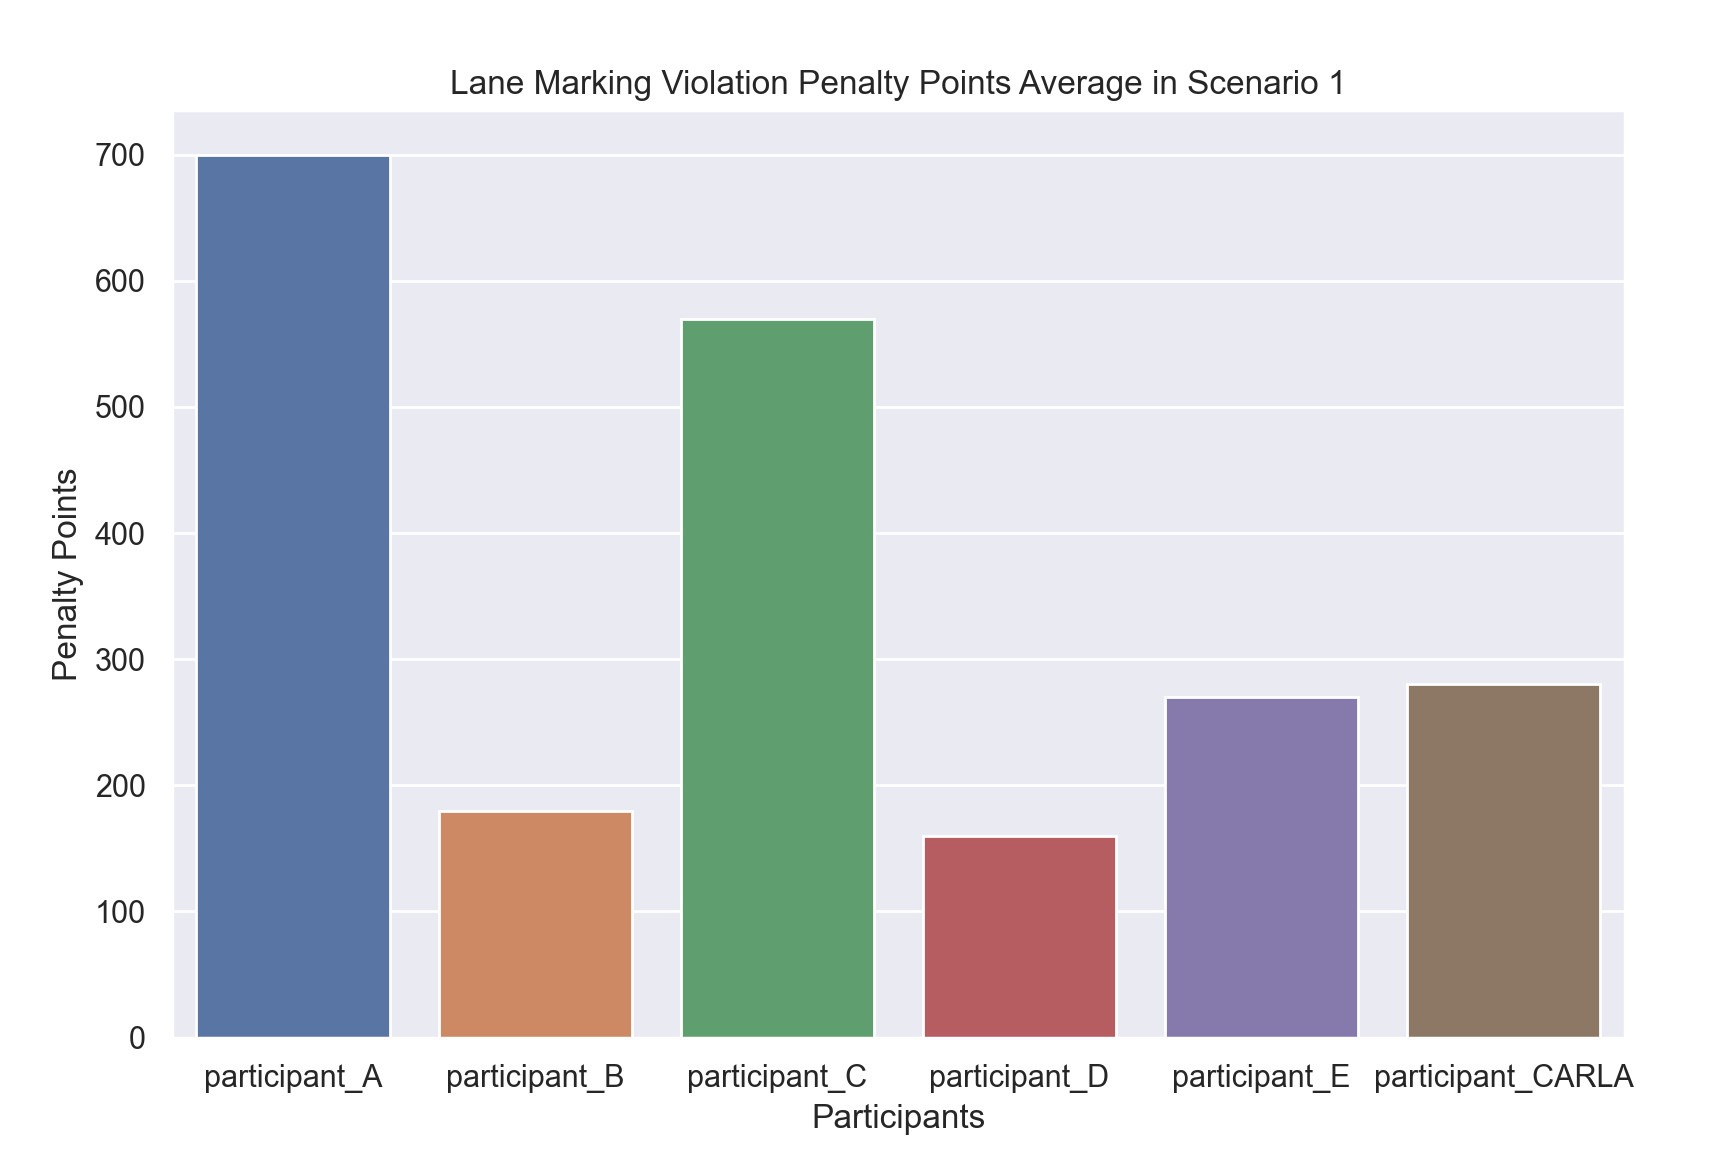
\includegraphics[width = 0.8\textwidth]{research_paper/Images/diagram_example.png}
    \caption{An example of a diagram}
    \label{fig:diagram_example}
\end{figure}

The third category of analysed data is locations where the violations occurred. Depending on the scenarios, participants and metrics specified in the analysis\_parameters.json file, the files in the points directory will differ. Taking a look at an example should clarify the purpose of this type of analysis. Suppose the parameters file specifies that the analysis should be performed on all the participants (listing their names) in scenario 1 and should consider the collisions only. The analysis tool would create a file points/scenario1\_collision\_data.xml containing all the locations where the collision occurred during the simulation runs of that particular scenario. If we then use the \textbf{draw\_map.sh} script and specify that file to be pictured, the view similar to the one in \autoref{fig:map_drawing} will appear on the screen.

\begin{figure} [h]
    \centering
    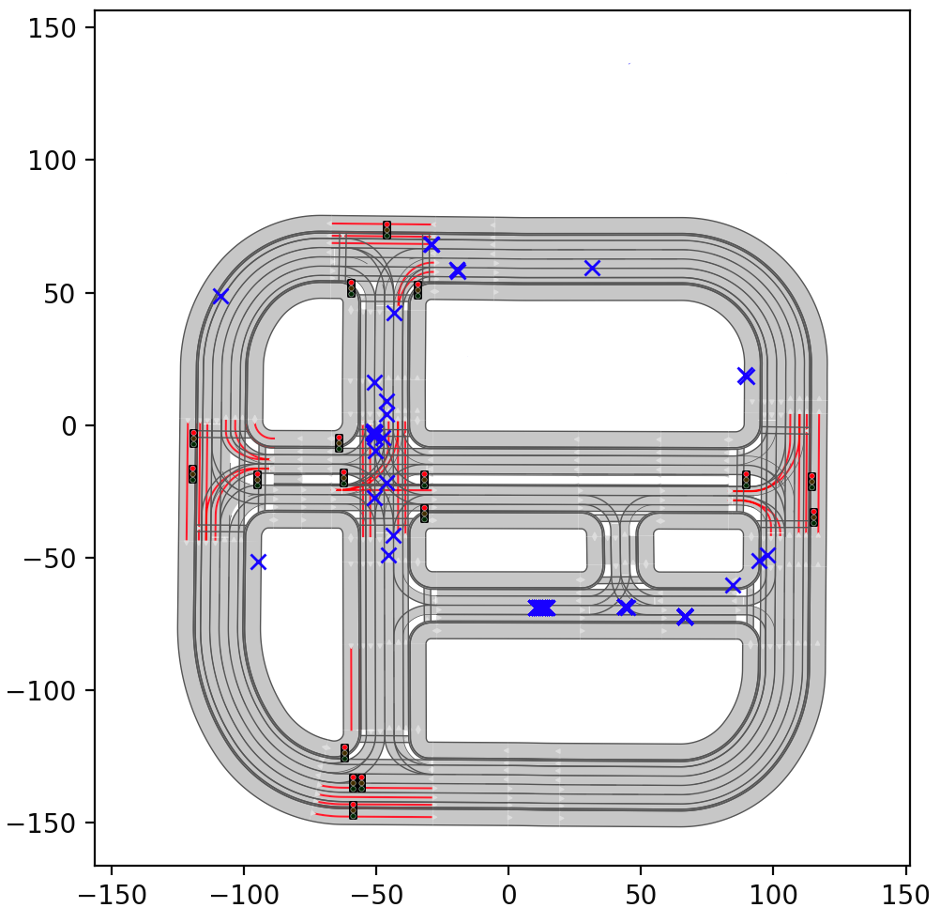
\includegraphics[width = 0.6\textwidth]{research_paper/Images/map_drawing.png}
    \caption{An example of a map with points marked}
    \label{fig:map_drawing}
\end{figure}

In this figure, the blue Xs indicate the places where the analysed participants made collisions. Information like this can help identify the places where the vehicle could not react on time or did not react appropriately, and the action resulted in a collision. With the help of the \textbf{replayer.sh} script, the simulations can be replayed to analyse the cause of the collision further and thus improve the AI model or simply observe the tendency. It is worth mentioning that the \textbf{draw\_map.sh} script can take two lists as parameters, depicting the points in red and blue Xs. This can be helpful in comparing the different participants or categories of participants.

As shown in the \autoref{fig:visualisation}, the map drawing process is facilitated by the CommonRoad Scenario Designer module \cite{maierhofer2021commonroad}. Note that this article uses a modified version of the CommonRoad Scenario Designer. This is due to the fact that the most recent version of it (version 0.6.0) did not have an option to provide a map and a list of points to be represented on the screen when launching the module. It only allows that after the tool was launched, and even then, it only allows for a single point to be marked on the screen. A few modifications were made to the module to launch the visualisation by just running a single command in the terminal. In addition, a bug was fixed not allowing to pass some arguments to the application. The owners of the project were informed about the error found. Because the CommonRoad Scenario Designer uses a different format for drawing the map, the OpenDRIVE files had to be converted to the CommonRoad map specification format. For this, a converter was created that can be found in the data/maps directory. The modified crdesigner module is located in the software/python\_libraries directory.

\section{Calculating the safety score} \label{sect-7.3}
In this section, we will briefly mention how the safety evaluation formula introduced in \autoref{sect-6.3} can be used to calculate the safety performance scores of participants in scenario simulations. For that, the \textbf{score\_calculator.py} script is used, which is located in the software/data\_analysis directory. The script takes two arguments: -p participant's name and -s scenario that the participant drove. Both arguments have to make a path in the data/recordings directory, meaning there must be data about the participant driving that particular scenario. An example of what is given to the user once the score-calculating script is run can be seen in \autoref{fig:score_calculation}. 

The script gathers data from the database, processes it, applies the formula and prints the score to the terminal, also indicating what is considered a perfect score. More about how to perform the data analysis, visualisation and score calculation is explained in \autoref{chap:b} where it is demonstrated how to use the project step by step. We will also come back to data analysis and score calculation in \autoref{chap:nine} when we analyse how human drivers and a CARLA agent performed in the scenarios.

\begin{figure} [h]
    \centering
    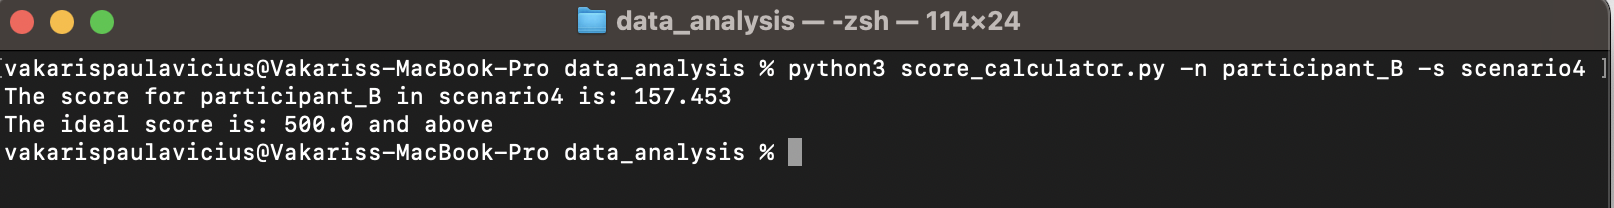
\includegraphics[width = \textwidth]{research_paper/Images/score_calculation.png}
    \caption{A score calculation example}
    \label{fig:score_calculation}
\end{figure}